% Generated by book/tools/notebook_to_tex.py. Do not edit by hand.

\chapter[보조 손실과 멀티태스크 학습 (Auxiliary Loss)]{보조 손실과 멀티태스크 학습 (Auxiliary Loss)}

\label{ch:14}

\markboth{보조 손실과 멀티태스크 학습 (Auxiliary Loss)}{보조 손실과 멀티태스크 학습 (Auxiliary Loss)}

\chaptermeta{14_auxiliary_loss/14_auxiliary_loss.ipynb}{https://colab.research.google.com/github/yoon-gu/neuqes-101/blob/master/14_auxiliary_loss/14_auxiliary_loss.ipynb}{다중 라벨 측면 분류에 별점 회귀 보조 헤드를 더해 결합 손실을 학습}



\index{1Auxiliary loss@Auxiliary loss}

\index{1multi task learning@multi-task learning}

\index{1combined loss@combined loss}

\index{1BCEWithLogitsLoss@BCEWithLogitsLoss}

\index{1MSELoss@MSELoss}

\index{1lambda@lambda}

\index{1auxiliary head@auxiliary head}

\index{1compute loss@compute\_loss}

\index{1DataCollatorWithPadding@DataCollatorWithPadding}

\index{1remove unused columns@remove\_unused\_columns}

\index{1custom Trainer@custom Trainer}

\index{0보조 손실@보조 손실}

\index{0멀티태스크 학습@멀티태스크 학습}

\index{0결합 손실@결합 손실}

\index{0보조 헤드@보조 헤드}

\index{0람다@람다}

\index{0커스텀 Trainer@커스텀 Trainer}

\index{0별점 보조 회귀@별점 보조 회귀}

\index{1nn Linear@nn.Linear}

\index{1torch nn functional@torch.nn.functional}

\index{1Trainer compute loss@Trainer.compute\_loss}

\index{1aux labels@aux\_labels}

\index{1lambda aux@lambda\_aux}

\index{1uncertainty weighting@uncertainty weighting}

\index{1custom data collator@custom data collator}

\index{1hidden states@hidden\_states}

\index{1return outputs@return\_outputs}

\index{0보조 라벨@보조 라벨}

\index{0불확실성 가중치@불확실성 가중치}

\index{0커스텀 데이터 콜레이터@커스텀 데이터 콜레이터}

\index{0은닉 상태@은닉 상태}



\section{변화추적표}

\begin{booktable}{14장 변화추적표}{tab:ch14-01}
\begin{adjustbox}{max width=\textwidth}
\begin{tabular}{@{}lllllll@{}}
\toprule
Ch & 모델 & 토크나이저 & 데이터 & Output Head & Activation & Loss \\
\midrule

9 & DistilBERT 파인튜닝 & WordPiece & Yelp 별점 & \inlinecode{Linear(H,\ 1)} & 없음 & \inlinecode{MSELoss} \\
13 & DistilBERT 파인튜닝 & WordPiece & Yelp + 측면 합성 & \inlinecode{Linear(H,\ 5)} & sigmoid (각각) & \inlinecode{BCEWithLogitsLoss} \\
\textbf{14 ← 여기} & DistilBERT + \textbf{보조 헤드} & WordPiece & Yelp + 측면 + \textbf{별점} & \textbf{메인(5) + 보조(1)} & 메인 sigmoid + 보조 없음 & \textbf{\inlinecode{BCE\ per-label\ +\ λ·MSE}} \\
15 (다음 Phase 2) & klue/bert-base & WordPiece (한국어) & NSMC & \inlinecode{Linear(H,\ 2)} & softmax & \inlinecode{CrossEntropyLoss} \\
\bottomrule
\end{tabular}
\end{adjustbox}
\end{booktable}

전체 20장 표는 \href{https://github.com/yoon-gu/neuqes-101\#챕터별-변화추적표}{루트 README.md}를 참고하세요.



\section{변경점: \ref{ch:13}장 대비}

\begin{booktable}{14장 변경점 요약}{tab:ch14-02}
\begin{adjustbox}{max width=\textwidth}
\begin{tabular}{@{}lll@{}}
\toprule
축 & \ref{ch:13}장 (multi-label) & \ref{ch:14}장 (multi-label + auxiliary) \\
\midrule

Task (메인) & 5라벨 multi-label & (그대로) \\
\inlinecode{num\_labels} & 5 & (그대로) \\
\inlinecode{problem\_type} & \inlinecode{multi\_label\_classification} & (그대로 --- 자동 매핑은 메인 loss 만 처리) \\
메인 활성화 / loss & per-label sigmoid / BCE & (그대로) \\
\textbf{보조 head} & 없음 & \textbf{새로 추가}: \inlinecode{Linear(H,\ 1)} linear regressor \\
\textbf{보조 라벨} & 없음 & \textbf{새로 추가}: 별점 0-1 스케일 (\inlinecode{label\ /\ 4}, 1★→0.0, 5★→1.0) \\
\textbf{보조 loss} & --- & \textbf{\inlinecode{MSELoss}} (\ref{ch:09}장 그대로) \\
\textbf{결합 loss} & \inlinecode{outputs.loss} 자동 & \textbf{\inlinecode{L\_main\ +\ λ·L\_aux}} 직접 계산 \\
\inlinecode{Trainer.compute\_loss} & 자동 (오버라이드 X) & \textbf{오버라이드 필수} \\
데이터 콜레이터 & \inlinecode{DataCollatorWithPadding} 자동 & \textbf{커스텀} --- \inlinecode{aux\_labels} 도 같이 batching \\
학습 hyperparams & (epoch=2, lr=2e-5, \ldots) & (그대로) \\
\bottomrule
\end{tabular}
\end{adjustbox}
\end{booktable}

\begin{quote}
\textbf{변하는 축 --- Loss 축 끝}: 메인 task와 모델 본체는 \emph{완전히 동일}, \emph{Loss에 보조 항이 가중합으로 추가} 됩니다. 실무에서 \emph{학습 데이터에 추가 신호가 있을 때} 이를 활용하는 정통 multi-task learning 패턴.
\end{quote}

\medskip\noindent\textbf{왜 보조 태스크가 메인 태스크에 도움이 되는가}

BERT 본체(67M 파라미터)가 \emph{공유} 되어 메인 헤드와 보조 헤드가 같은 768-dim CLS 표현을 입력으로 받습니다. 보조 task가 메인과 \emph{부분적으로 상관} 이면 보조 학습이 본체를 \emph{더 일반적인 표현} 으로 끌고 가서 메인 정확도까지 올라갑니다. 다음 섹션에서 \emph{어떤 상황에서 왜 도움이 되는지} 다섯 갈래로 자세히 봅니다.



\section{왜 보조 손실인가}

코드를 짜기 전에 \emph{언제·왜} 보조 loss를 쓰는지 정리합니다. 이 장의 셋업이 다섯 동기 중 어디에 해당하는지 의식적으로 짚어 두면 학습 결과를 \emph{예측하고 해석} 하는 감각이 생깁니다.

\medskip\noindent\textbf{정규화}

메인 task만 학습하면 모델이 \emph{그 task 한정} 으로 과적합됩니다. 보조 task가 BERT 본체를 \emph{더 일반적인} 표현으로 끌고 가서 메인에서도 일반화가 좋아집니다. Dropout과 비슷한 효과지만 \textbf{데이터 신호} 로 정규화하는 점이 다릅니다.

\begin{quote}
\textbf{이 장의 주된 목적이 이거.} 측면 라벨이 키워드 매칭으로 \emph{합성} 되어 노이즈가 큰데, 별점은 사용자가 \emph{직접} 매긴 깨끗한 ground truth. 별점 회귀를 보조로 두면 BERT가 \emph{과도하게 키워드 매칭에 맞추는} 걸 막아 일반화에 도움.
\end{quote}

\medskip\noindent\textbf{데이터 효율}

메인 task의 라벨링 비용이 큰데 \emph{부가 신호} (별점, 작성일, 길이, 작성자, 카테고리 \ldots)가 데이터에 \emph{공짜로 함께 있는} 시나리오. 메인 라벨이 부족해도 보조 신호를 \emph{동시에} 학습하면 BERT 본체가 더 풍부하게 학습됩니다.

\Needspace{6\baselineskip}
\begin{lstlisting}
main_label = expensive_human_annotated_aspects
aux_label  = star_rating
\end{lstlisting}

\medskip\noindent\textbf{도메인 지식 주입}

알고 있는 \emph{구조적 정보} 를 보조 task로 모델에 \emph{강제} 학습시키는 방법.

\begin{booktable}{14장 (3) 도메인 지식 주입 (Inductive Bias) 표}{tab:ch14-03}
\begin{adjustbox}{max width=\textwidth}
\begin{tabular}{@{}lll@{}}
\toprule
메인 task & 보조 task & 주입되는 지식 \\
\midrule

NER (개체명 추출) & POS tagging (품사) & 구문 구조 \\
객체 검출 (위치+범주) & 세그멘테이션 (경계) & 위치-경계 일관성 \\
한국어 분류 & 한자 음운 예측 & 어휘 형태소 구조 \\
영화 리뷰 감성 & 영화 장르 분류 & 장르별 감성 표현 차이 \\
\bottomrule
\end{tabular}
\end{adjustbox}
\end{booktable}

연구·실무에서 \emph{어떤 보조를 써야 메인이 좋아질지} 는 도메인 지식의 영역. 입문 수준에선 \emph{데이터에 있는 신호 중 메인과 양의 상관} 인 걸 골라 시작.

\medskip\noindent\textbf{학습 안정화}

깊은 네트워크에서 gradient가 \emph{최하위 층까지 도달하지 못하는} 문제를 보조 분류 헤드를 \emph{중간 층에} 달아 해결한 패턴. \textbf{GoogLeNet (2014)} 의 intermediate auxiliary classifiers 가 원조.

\begin{quote}
BERT는 12-24 layer로 \emph{그리} 깊지 않아 이 목적은 약합니다. CNN 100+ layer (ResNet-152) 시대의 잔재. 입문 수준에선 \emph{왜 이런 패턴이 historically 등장했는지} 만 알아두면 충분.
\end{quote}

\medskip\noindent\textbf{운영 시점의 멀티태스크}

추론 시점에 \emph{두 task 결과가 모두 필요} 한 경우 --- 한 번의 forward로 측면 분류 + 별점 예측을 동시에 받기. 엄밀히 말하면 \emph{auxiliary} 가 아니라 \emph{joint training} 이 됩니다.

\begin{quote}
\ref{ch:14}장는 \emph{auxiliary} 패턴이라 추론 시 보조 헤드를 \emph{호출하지 않습니다}. 별점 회귀는 학습 정규화 용도로만 사용. 운영에서 별점 예측이 필요하면 \emph{auxiliary} 가 아니라 \emph{joint multi-task} 를 의도적으로 설계.
\end{quote}

\begin{center}\rule{0.5\linewidth}{0.5pt}\end{center}

\medskip\noindent\textbf{\ref{ch:14}장의 위치}

이 장의 셋업은 다섯 중 두 가지에 해당합니다:

\begin{itemize}
\tightlist
\item
  \textbf{(1) 정규화}: 합성 측면 라벨의 노이즈를 깨끗한 별점 신호로 정규화 --- 주된 효과
\item
  \textbf{(2) 데이터 효율}: 별점은 Yelp 데이터에 \emph{이미} 있어 추가 라벨링 비용 0
\end{itemize}

학습 결과를 해석할 때 두 효과가 \emph{같이} 나타날 거라 예측. 메인 F1이 1-3\%p 올라가면 정규화 효과가 두드러진 것, 5\%p 이상이면 데이터 효율 + 정규화가 합쳐진 것.

\begin{center}\rule{0.5\linewidth}{0.5pt}\end{center}

\medskip\noindent\textbf{보조 손실이 해로운 경우}

\begin{booktable}{14장 언제 안 쓰나 - 보조가 해로운 경우 표}{tab:ch14-04}
\begin{adjustbox}{max width=\textwidth}
\begin{tabular}{@{}lll@{}}
\toprule
조건 & 결과 & 진단 신호 \\
\midrule

보조가 메인과 \emph{반대 신호} & gradient 충돌, 학습 발산 & 두 loss가 \emph{둘 다 정체}, λ 키울수록 메인 metric 하락 \\
보조 라벨이 \emph{극도로 sparse} & 학습 신호 부족 & aux loss가 거의 0, 메인엔 영향 없음 \\
보조가 메인보다 \emph{훨씬 어려움} & 학습량 부족으로 둘 다 학습 안 됨 & 두 metric 모두 baseline 이하 \\
λ 튜닝 비용을 감당 못 함 & 잘못된 λ로 메인이 망가짐 & 단순히 단일 task가 더 안전 \\
\bottomrule
\end{tabular}
\end{adjustbox}
\end{booktable}

\medskip\noindent\textbf{역사적 교훈}

BERT 자체가 \emph{MLM + NSP (Next Sentence Prediction)} 이라는 멀티태스크 사전학습으로 만들어졌습니다 --- MLM이 메인, NSP가 보조였던 셈. 그런데 \textbf{RoBERTa (2019)} 가 \emph{NSP를 빼면 오히려 성능이 좋아진다} 는 걸 발견하고 NSP를 제거. 이후 거의 모든 BERT 후속 모델 (DeBERTa, ELECTRA \ldots)이 NSP 없이 학습됨.

\begin{quote}
\textbf{시사점}: 보조 task가 \emph{직관적으로} 도움 될 것 같아도 \emph{실제로 도움이 되는지는 측정} 해야 합니다. 그래서 이 장의 §8 클라이맥스가 λ=0 baseline과의 \emph{직접 비교} 인 것 --- “직관” 대신 “측정”.
\end{quote}



\section{\texorpdfstring{손실 노트}{손실 노트}}

\begin{equation}
\label{eq:ch14-01}
L = \underbrace{\frac{1}{N \cdot K}\sum_{i,k}\text{BCE}(z_{i,k}^{main}, y_{i,k}^{main})}_{L_\text{main}: \text{측면 BCE per-label}} + \lambda \cdot \underbrace{\frac{1}{N}\sum_{i}(z_{i}^{aux} - y_{i}^{aux})^2}_{L_\text{aux}: \text{별점 MSE}}
\end{equation}

식~\eqref{eq:ch14-01}은 정답 라벨과 예측 확률 사이의 Binary Cross-Entropy를 정의합니다.

\begin{itemize}
\tightlist
\item
  \(z^\text{main} \in \mathbb{R}^5\) --- 측면 logit 5개, sigmoid 후 BCE.
\item
  \(z^\text{aux} \in \mathbb{R}\) --- 별점 회귀 logit (활성화 없음, 직접 MSE).
\item
  \(\lambda\) --- 보조 loss의 가중치 (hyperparameter, 보통 0.1-10 범위 탐색).
\end{itemize}

\textbf{λ 선택 가이드 --- 숫자로 감 잡기}

\begin{booktable}{14장 손실 노트 표}{tab:ch14-05}
\begin{adjustbox}{max width=\textwidth}
\begin{tabular}{@{}lll@{}}
\toprule
λ & 의미 & 효과 (예상) \\
\midrule

0.0 & 보조 loss 무시 & \ref{ch:13}장과 \emph{완전히 동일} (이 장 §5 baseline) \\
0.1 & 보조 \emph{약하게} 반영 & 메인이 압도적, 보조는 살짝 정규화 효과 \\
1.0 & \textbf{보조와 메인 \emph{동등} 가중} & 표준 시작점. 두 task가 균형 잡혀 학습 \\
5.0 & 보조 우세 & 보조 task가 학습 방향을 지배 --- 메인 task 성능 떨어질 수 있음 \\
10+ & 보조 절대 우세 & 메인 task 신호가 거의 묻힘. 권장 안 됨 \\
\bottomrule
\end{tabular}
\end{adjustbox}
\end{booktable}

이 장에선 \textbf{λ=1} 로 학습하고 λ=0 baseline과 비교. 실무에선 validation set에서 λ를 grid search (0.1, 0.3, 1, 3, 10).

\textbf{숫자로 감 잡기 (단일 샘플)} --- 측면 multi-hot \(\mathbf{y}^\text{main} = [1, 0, 1, 0, 1]\), 별점 보조 라벨 \(y^\text{aux} = 0.75\) (4★/4):

\begin{booktable}{14장 손실 노트 표}{tab:ch14-06}
\begin{adjustbox}{max width=\textwidth}
\begin{tabular}{@{}ll@{}}
\toprule
단계 & 값 \\
\midrule

\(L_\text{main}\) (\ref{ch:13}장의 BCE per-label 평균) & 0.45 \\
\(L_\text{aux}\) (\((z^\text{aux} - 0.75)^2\), 가정 \(z^\text{aux} = 0.55\)) & \((0.55 - 0.75)^2 = 0.04\) \\
\(L\) (λ=1) & \(0.45 + 1 \cdot 0.04 = 0.49\) \\
\(L\) (λ=10) & \(0.45 + 10 \cdot 0.04 = 0.85\) ← 보조 항이 메인보다 큼 \\
\bottomrule
\end{tabular}
\end{adjustbox}
\end{booktable}

λ가 너무 크면 \emph{메인 신호 자체가 보조에 묻힙니다}. 반대로 너무 작으면 \emph{보조 신호가 학습에 영향 안 줌}. λ=1이 균형의 기본 출발점.



\section{토크나이저 노트}

\ref{ch:13}장과 완전히 동일 --- \inlinecode{distilbert-base-uncased} WordPiece, \inlinecode{max\_length=128}. 토크나이저는 \emph{라벨에 무관} 합니다. 보조 라벨이 추가됐다고 토큰화가 바뀌지는 않음 --- 별점 정수가 \emph{float 값으로 한 칸 더} 추가될 뿐.

\begin{previewBox}{미리보기}
\textbf{다음 장(15장)부터 Phase 2}: 같은 셋업을 한국어 BERT(\inlinecode{klue/bert-base})에서 다시. 토크나이저가 \emph{영어 WordPiece → 한국어 WordPiece} 로 바뀌는 게 변화의 본질.
\end{previewBox}



\Needspace{8\baselineskip}
\begin{lstlisting}
!pip install -q transformers datasets
\end{lstlisting}

\begin{codeRead}
\textbf{1행}의 \inlinecode{!pip install -q transform...}에서는 Colab 실행에 필요한 패키지를 설치합니다.
\end{codeRead}



\Needspace{26\baselineskip}
\begin{lstlisting}
import warnings
warnings.filterwarnings("ignore")

import re
import numpy as np
import pandas as pd
import matplotlib.pyplot as plt
import seaborn as sns
import torch
import torch.nn as nn
import torch.nn.functional as F
from datasets import load_dataset
from transformers import (
    AutoTokenizer, AutoModelForSequenceClassification,
    Trainer, TrainingArguments,
    DataCollatorWithPadding,
)
from sklearn.metrics import (
    precision_recall_fscore_support, classification_report,
    roc_auc_score, hamming_loss, mean_squared_error, r2_score,
)

plt.rcParams["axes.unicode_minus"] = False

print(f"PyTorch:        {torch.__version__}")
print(f"CUDA available: {torch.cuda.is_available()}")
if torch.cuda.is_available():
    print(
        f"GPU:             "
        f"{torch.cuda.get_device_name(0)}"
    )
else:
    print(
        "Warning: CPU runtime — training will be very "
        "slow. Switch to T4 recommended."
    )
\end{lstlisting}

\begin{codeRead}
\inlinecode{numpy, pandas, matplotlib, PyTorch, datasets} 같은 주요 패키지를 불러옵니다.
\end{codeRead}



\textbf{baseline VRAM}:



\Needspace{8\baselineskip}
\begin{lstlisting}
!nvidia-smi
\end{lstlisting}

\begin{codeRead}
\textbf{1행}의 \inlinecode{!nvidia-smi}에서는 앞 단계에서 만든 값을 바탕으로 다음 계산을 수행합니다.
\end{codeRead}



\section{데이터 준비}

\ref{ch:13}장의 측면 합성 라벨을 그대로 쓰고, \textbf{별점 보조 회귀 라벨} 을 추가합니다. 별점은 1-5 정수지만 회귀 헤드와 MSE를 자연스럽게 쓰기 위해 \emph{0-1 스케일} 로 변환만 해 둡니다 (학습 정규화 효과를 위한 데이터 가공이 아니라, 단순히 단위만 맞추는 작업).

\begin{itemize}
\tightlist
\item
  메인 라벨 \(\mathbf{y}^\text{main} \in \{0, 1\}^5\) --- 측면 multi-hot.
\item
  보조 라벨 \(y^\text{aux} = \text{label} / 4 \in [0, 1]\) --- 1★ → 0.0, 5★ → 1.0.
\end{itemize}



\Needspace{26\baselineskip}
\begin{lstlisting}
ASPECT_KEYWORDS = {
    "food": ["food", "meal", "dish", "taste", "delicious", "flavor", "menu",
             "cuisine", "tasty", "yummy", "spicy", "sweet", "salty", "fresh"],
    "service": ["service", "staff", "waiter", "waitress", "server", "friendly",
                "rude", "attentive", "host", "helpful", "polite", "manager"],
    "price": ["price", "cheap", "expensive", "value", "worth", "cost",
              "money", "afford", "overpriced", "pricey", "deal", "bargain"],
    "ambiance": ["atmosphere", "ambiance", "decor", "music", "vibe", "cozy",
                 "noisy", "quiet", "lighting", "interior", "comfortable", "loud"],
    "location": ["location", "parking", "area", "neighborhood", "access",
                 "downtown", "convenient", "spot"],
}
ASPECTS = list(ASPECT_KEYWORDS.keys())
K = len(ASPECTS)

def extract_aspects(text: str) -> list[float]:
    text_lower = text.lower()
    return [
        float(any(re.search(rf"\b{re.escape(kw)}\b", text_lower) for kw in keywords))
        for keywords in ASPECT_KEYWORDS.values()
    ]

print(f"K (aspects): {K}, aspects: {ASPECTS}")
\end{lstlisting}



\Needspace{26\baselineskip}
\begin{lstlisting}
tokenizer = AutoTokenizer.from_pretrained("distilbert-base-uncased")

ds = load_dataset("yelp_review_full")
train_full = ds["train"].shuffle(seed=42).select(range(5000))
eval_full  = ds["test"].shuffle(seed=42).select(range(1000))

def attach_aspects_and_aux(batch):
    batch["aspects"] = [extract_aspects(t) for t in batch["text"]]

    batch["aux_score"] = [float(l) / 4.0 for l in batch["label"]]
    return batch

train_full = train_full.map(
    attach_aspects_and_aux,
    batched=True,
)
eval_full  = eval_full.map(
    attach_aspects_and_aux,
    batched=True,
)

print(f"train: {len(train_full)}, eval: {len(eval_full)}")
print(f"\nFirst sample:")
print(f"  text: {train_full[0]['text'][:120]}...")
print(
    f"  aspects (multi-hot): "
    f"{train_full[0]['aspects']}"
)
print(
    f"  aux_score (star/4): {train_full[0]['aux_score']:.2f}  (star = "
    f"{train_full[0]['label'] + 1})"
)
\end{lstlisting}



\Needspace{22\baselineskip}
\begin{lstlisting}
import numpy as np
aux_train = np.array(train_full["aux_score"])
print(
    f"aux score range: [{aux_train.min():.2f}, "
    f"{aux_train.max():.2f}]"
)
print(
    f"aux score mean: {aux_train.mean():.3f}, std: "
    f"{aux_train.std():.3f}"
)
print(f"\nAux score distribution (train):")
for v in [0.0, 0.25, 0.5, 0.75, 1.0]:
    cnt = (np.isclose(aux_train, v)).sum()
    star = int(v * 4) + 1
    print(
        f"  {v:.2f}  (star {star}): {cnt} samples ("
        f"{cnt/len(aux_train):.1%})"
    )
\end{lstlisting}



\section{토큰화}

\inlinecode{tokenize\_fn} 이 두 라벨을 모두 attach. 메인은 \inlinecode{labels} (multi-hot float), 보조는 \inlinecode{aux\_labels} (float scalar).



\Needspace{26\baselineskip}
\begin{lstlisting}
def tokenize_fn(batch):
    out = tokenizer(
        batch["text"],
        truncation=True,
        max_length=128,
    )
    out["labels"]     = [list(map(float, a)) for a in batch["aspects"]]
    out["aux_labels"] = [float(s) for s in batch["aux_score"]]
    # float scalar
    return out

train_tok = train_full.map(tokenize_fn, batched=True).remove_columns(
    ["text", "label", "aspects", "aux_score"]
)
eval_tok  = eval_full.map(tokenize_fn,  batched=True).remove_columns(
    ["text", "label", "aspects", "aux_score"]
)

print(train_tok)
print(f"\nFirst sample labels: {train_tok[0]['labels']}")
print(
    f"First sample aux_labels: "
    f"{train_tok[0]['aux_labels']:.2f}"
)
\end{lstlisting}



\section{\texorpdfstring{커스텀 Data Collator}{커스텀 Data Collator}}

기본 \inlinecode{DataCollatorWithPadding} 은 input\_ids·attention\_mask·labels 만 알고 있어 \emph{추가 라벨} 은 통과시키지 못합니다. 한 줄짜리 wrapper로 \inlinecode{aux\_labels} 를 텐서로 만들어 batch에 추가합니다.



\Needspace{26\baselineskip}
\begin{lstlisting}
class AuxCollator:
    def __init__(self, tokenizer):
        self.base = DataCollatorWithPadding(tokenizer)

    def __call__(self, features):

        aux = torch.tensor(
            [f.pop("aux_labels") for f in features],
            dtype=torch.float,
        )

        batch = self.base(features)

        batch["labels"] = batch["labels"].float()

        batch["aux_labels"] = aux
        return batch

collator = AuxCollator(tokenizer)

sample_features = [dict(train_tok[i]) for i in range(4)]
batch = collator(sample_features)
print("Batch keys:", list(batch.keys()))
for k, v in batch.items():
    print(
        f"  {k}: shape={tuple(v.shape)}, dtype="
        f"{v.dtype}"
    )
\end{lstlisting}



\section{모델 셋업}

\inlinecode{AutoModelForSequenceClassification} (\ref{ch:13}장과 \emph{완전히 동일}) 을 로드한 뒤 \inlinecode{model.aux\_head\ =\ nn.Linear(...)} 한 줄로 보조 헤드를 \emph{모델 객체에 attach}. 이후 \inlinecode{Trainer.compute\_loss} 가 메인 출력 + 보조 헤드를 동시에 사용해 결합 loss 를 계산합니다.



\Needspace{26\baselineskip}
\begin{lstlisting}
def make_model():
    m = AutoModelForSequenceClassification.from_pretrained(
        "distilbert-base-uncased",
        num_labels=K,
        problem_type="multi_label_classification",
        id2label={i: a for i, a in enumerate(ASPECTS)},
        label2id={a: i for i, a in enumerate(ASPECTS)},
    )

    H = m.config.dim   # distilbert hidden size
    m.aux_head = nn.Linear(H, 1)

    return m

model = make_model()

def param_summary(m):
    total     = sum(p.numel() for p in m.parameters())
    trainable = sum(p.numel() for p in m.parameters() if p.requires_grad)
    aux_only  = sum(
        p.numel() for n,
        p in m.named_parameters() if n.startswith("aux_head"),
    )
    return total, trainable, aux_only

total, trainable, aux_only = param_summary(model)
print(
    f"Parameters:           {total:>13,}  ("
    f"{total/1e6:.1f} M)"
)
print(
    f"Trainable parameters: {trainable:>13,}  ("
    f"{trainable/total:.1%})"
)
print(
    f"Aux head parameters:  {aux_only:>13,}  ("
    f"{aux_only/total:.4%})"
)
print(f"Main classifier:      {model.classifier}")
print(f"Aux head:             {model.aux_head}")
\end{lstlisting}



\textbf{보조 헤드는 \textasciitilde770개 파라미터} --- 768→1 Linear의 weight + bias. 전체 67M 의 \emph{0.001\%}. 이 \emph{미세한 추가 자유도} 만으로 멀티태스크 학습이 동작합니다.



\section{\texorpdfstring{커스텀 Trainer}{커스텀 Trainer}}

핵심 로직 (코드 한 줄로 요약):

\Needspace{6\baselineskip}
\begin{lstlisting}
loss = outputs.loss + λ · MSE(aux_head(CLS), aux_labels)
\end{lstlisting}

\begin{itemize}
\tightlist
\item
  \inlinecode{outputs.loss} 는 \inlinecode{problem\_type="multi\_label\_classification"} 자동 매핑으로 이미 BCE per-label 평균이 계산됨.
\item
  보조 loss는 우리가 \emph{직접 계산} --- \inlinecode{output\_hidden\_states=True} 로 받은 마지막 layer의 CLS 표현을 \inlinecode{aux\_head} 에 통과.
\end{itemize}



\Needspace{26\baselineskip}
\begin{lstlisting}
from transformers.modeling_outputs import SequenceClassifierOutput

class AuxTrainer(Trainer):
    def __init__(self, *args, lambda_aux: float = 1.0, **kwargs):
        super().__init__(*args, **kwargs)
        self.lambda_aux = lambda_aux

    def compute_loss(self, model, inputs, return_outputs=False, num_items_in_batch=None):
        aux_labels = inputs.pop("aux_labels")

        outputs = model(
            **inputs,
            output_hidden_states=True,
        )
        main_loss = outputs.loss

        cls = outputs.hidden_states[-1][:, 0, :]   # (
            B,
            768,
        )
        aux_logits = model.aux_head(cls).squeeze(-1)
        # (B,)
        aux_loss = F.mse_loss(
            aux_logits,
            aux_labels.float(),
        )

        loss = main_loss + self.lambda_aux * aux_loss

        if return_outputs:

            clean = SequenceClassifierOutput(
                loss=loss,
                logits=outputs.logits,
            )
            return (loss, clean)
        return loss

print(
    "AuxTrainer 정의 완료 — Trainer 의 compute_loss 만 "
    "교체."
)
\end{lstlisting}



\textbf{평가용 metric 함수} --- 메인 (\ref{ch:13}장과 동일) + 보조 (RMSE, R², Pearson r). 보조 logit 추출은 \inlinecode{Trainer.predict()} 가 메인 logits 만 반환하기 때문에 별도 단계로 빼서 처리.



\Needspace{26\baselineskip}
\begin{lstlisting}
def compute_metrics_main(eval_pred):

    logits, labels = eval_pred

    if isinstance(logits, tuple):
        logits = logits[0]
    probs = 1.0 / (1.0 + np.exp(-logits))
    preds = (probs >= 0.5).astype(int)

    out = {"hamming_loss": float(hamming_loss(labels, preds))}
    p_mi, r_mi, f1_mi, _ = precision_recall_fscore_support(
        labels, preds, average="micro", zero_division=0,
    )
    out["micro_f1"] = float(f1_mi)
    out["micro_precision"] = float(p_mi)
    out["micro_recall"]    = float(r_mi)
    p_ma, r_ma, f1_ma, _ = precision_recall_fscore_support(
        labels, preds, average="macro", zero_division=0,
    )
    out["macro_f1"] = float(f1_ma)
    out["macro_precision"] = float(p_ma)
    out["macro_recall"]    = float(r_ma)
    try:
        out["macro_auc"] = float(roc_auc_score(labels, probs, average="macro"))
    except ValueError:
        out["macro_auc"] = float("nan")
    return out
\end{lstlisting}



\section{학습}

\ref{ch:13}장과 동일한 hyperparams. \inlinecode{AuxTrainer} + \inlinecode{lambda\_aux=1.0}.



\Needspace{26\baselineskip}
\begin{lstlisting}
LAMBDA_AUX = 1.0

training_args = TrainingArguments(
    output_dir="./ch14_aux_output",
    num_train_epochs=2,
    per_device_train_batch_size=16,
    per_device_eval_batch_size=32,
    learning_rate=2e-5,
    fp16=True,
    eval_strategy="epoch",
    logging_steps=50,
    save_strategy="no",
    report_to="none",
    seed=42,
    remove_unused_columns=False,
)

trainer_aux = AuxTrainer(
    model=model,
    args=training_args,
    train_dataset=train_tok,
    eval_dataset=eval_tok,
    data_collator=collator,
    processing_class=tokenizer,
    compute_metrics=compute_metrics_main,
    lambda_aux=LAMBDA_AUX,
)

train_result_aux = trainer_aux.train()
print(
    f"\nWith-aux training done — mean train loss: "
    f"{train_result_aux.training_loss:.4f}"
)
\end{lstlisting}



\textbf{중요: \inlinecode{remove\_unused\_columns=False}} --- Trainer는 기본으로 \emph{model.forward 시그니처에 없는 컬럼} 을 제거합니다. \inlinecode{aux\_labels} 는 모델 시그니처에 없어 자동 제거되면 우리 \inlinecode{compute\_loss} 가 받을 수 없습니다. 이 옵션을 꺼야 함.



\Needspace{8\baselineskip}
\begin{lstlisting}
!nvidia-smi
\end{lstlisting}



\section{평가}

메인 metric 은 자동으로 계산됨 (\inlinecode{compute\_metrics}). 보조 metric (RMSE, R², Pearson r) 은 별도 forward로 보조 logits 를 추출해 측정.



\Needspace{9\baselineskip}
\begin{lstlisting}
eval_metrics_aux = trainer_aux.evaluate()
print("With-aux (λ=1) — main task metrics:")
for k, v in eval_metrics_aux.items():
    if k.startswith("eval_") and isinstance(v, float):
        print(f"  {k:>22}: {v:.4f}")
\end{lstlisting}



\Needspace{26\baselineskip}
\begin{lstlisting}
@torch.no_grad()
def aux_predictions(trainer, dataset, batch_size=64):
    trainer.model.eval()
    device = trainer.model.device
    aux_preds, aux_true = [], []
    for i in range(0, len(dataset), batch_size):
        batch_features = [dict(dataset[j]) for j in range(i, min(i + batch_size, len(dataset)))]
        batch = trainer.data_collator(batch_features)
        batch_on_device = {k: v.to(device) for k, v in batch.items()}
        aux_lbl = batch_on_device.pop("aux_labels").cpu().numpy()
        out = trainer.model(**{k: v for k, v in batch_on_device.items() if k != "labels"},
                            output_hidden_states=True)
        cls = out.hidden_states[-1][:, 0, :]
        aux_logits = trainer.model.aux_head(cls).squeeze(-1).cpu().numpy()
        aux_preds.extend(aux_logits.tolist())
        aux_true.extend(aux_lbl.tolist())
    return np.array(aux_preds), np.array(aux_true)

aux_preds_aux, aux_true = aux_predictions(
    trainer_aux,
    eval_tok,
)
rmse_aux = float(np.sqrt(mean_squared_error(aux_true, aux_preds_aux)))
r2_aux   = float(r2_score(aux_true, aux_preds_aux))
pear_aux = float(np.corrcoef(aux_true, aux_preds_aux)[0, 1])

print(
    "\nWith-aux (λ=1) — aux task metrics (star "
    "regression, 0-1 scale):"
)
print(f"  RMSE:    {rmse_aux:.4f}")
print(f"  R^2:     {r2_aux:.4f}")
print(f"  Pearson: {pear_aux:.4f}")
\end{lstlisting}



\Needspace{14\baselineskip}
\begin{lstlisting}
preds_output_aux = trainer_aux.predict(eval_tok)
logits_aux = preds_output_aux.predictions
if isinstance(logits_aux, tuple):
    logits_aux = logits_aux[0]
labels_eval = preds_output_aux.label_ids.astype(int)
probs_aux = 1.0 / (1.0 + np.exp(-logits_aux))
preds_main_aux = (probs_aux >= 0.5).astype(int)

print(f"Main logits shape: {logits_aux.shape}")
print(f"Eval samples:      {len(labels_eval)}")
\end{lstlisting}



\section{lambda=0 기준선 비교}

같은 코드를 \inlinecode{lambda\_aux=0.0} 으로 한 번 더 돌립니다. 그러면 보조 loss 의 gradient 가 0이 되어 메인 task만 학습되는 상태 = \textbf{\ref{ch:13}장과 정확히 동일한 학습 결과}. (보조 헤드는 학습되긴 하지만 메인 학습엔 영향 없음.)

\begin{quote}
의도적으로 \emph{\ref{ch:13}장 노트북을 따로 돌리지 않고} 이 셀에서 baseline을 다시 만듭니다 --- 비교가 \emph{같은 노트북·같은 환경} 안에서 self-contained 하도록.
\end{quote}



\Needspace{26\baselineskip}
\begin{lstlisting}
model_no_aux = make_model()

training_args_no_aux = TrainingArguments(
    output_dir="./ch14_baseline_output",
    num_train_epochs=2,
    per_device_train_batch_size=16,
    per_device_eval_batch_size=32,
    learning_rate=2e-5,
    fp16=True,
    eval_strategy="epoch",
    logging_steps=50,
    save_strategy="no",
    report_to="none",
    seed=42,
    remove_unused_columns=False,
)

trainer_no_aux = AuxTrainer(
    model=model_no_aux,
    args=training_args_no_aux,
    train_dataset=train_tok,
    eval_dataset=eval_tok,
    data_collator=collator,
    processing_class=tokenizer,
    compute_metrics=compute_metrics_main,
    lambda_aux=0.0,
)

train_result_no_aux = trainer_no_aux.train()
print(
    f"\nNo-aux (λ=0) baseline training done — mean train loss: "
    f"{train_result_no_aux.training_loss:.4f}"
)
\end{lstlisting}



\Needspace{16\baselineskip}
\begin{lstlisting}
eval_metrics_no_aux = trainer_no_aux.evaluate()
print("No-aux (λ=0) baseline — main task metrics:")
for k, v in eval_metrics_no_aux.items():
    if k.startswith("eval_") and isinstance(v, float):
        print(f"  {k:>22}: {v:.4f}")

preds_output_no_aux = trainer_no_aux.predict(eval_tok)
logits_no_aux = preds_output_no_aux.predictions
if isinstance(logits_no_aux, tuple):
    logits_no_aux = logits_no_aux[0]
probs_no_aux = 1.0 / (1.0 + np.exp(-logits_no_aux))
preds_main_no_aux = (probs_no_aux >= 0.5).astype(int)
\end{lstlisting}



\subsection{메인 지표 비교}



\Needspace{25\baselineskip}
\begin{lstlisting}
m_aux    = {k.replace(
    "eval_",
    ""): v for k,
    v in eval_metrics_aux.items(,
)
            if k.startswith("eval_") and isinstance(v, float)}
m_no_aux = {k.replace(
    "eval_",
    ""): v for k,
    v in eval_metrics_no_aux.items(,
)
            if k.startswith("eval_") and isinstance(v, float)}

common = [k for k in m_aux if k in m_no_aux]
cmp = pd.DataFrame({
    "metric":             common,
    "no aux (lambda=0)":  [m_no_aux[k] for k in common],
    "with aux (lambda=1)":[m_aux[k]    for k in common],
})
cmp["delta (aux - no_aux)"] = cmp["with aux (lambda=1)"] - cmp["no aux (lambda=0)"]
print(cmp.round(4).to_string(index=False))
\end{lstlisting}



\textbf{해석 가이드}

\begin{itemize}
\tightlist
\item
  \inlinecode{delta} \textgreater{} 0 --- 보조 loss 가 메인 task 에 \emph{도움} 이 됨 (멀티태스크의 정통 효과).
\item
  \inlinecode{delta} \textless{} 0 --- 보조 loss 가 메인 task 를 \emph{방해} 함 (λ가 너무 큼 / 보조 task 가 메인과 상관 약함).
\item
  \inlinecode{delta} ≈ 0 --- 별 영향 없음 (보조 신호가 메인 표현에 의미 없는 추가).
\end{itemize}

별점은 측면 분포와 \emph{부분적으로} 상관 (긍정 측면 → 높은 별점) 이라 \emph{작은 양의 delta} 가 자연스러운 결과. 0.5\%p 정도면 노이즈일 수 있고, 1-2\%p 면 의미 있는 효과.



\subsection{라벨별 F1 비교}



\Needspace{26\baselineskip}
\begin{lstlisting}
def per_label_f1(Y_true, Y_pred):
    f1s = []
    for k in range(K):
        _, _, f1, _ = precision_recall_fscore_support(
            Y_true[:, k], Y_pred[:, k], average="binary", zero_division=0,
        )
        f1s.append(float(f1))
    return f1s

f1_no_aux = per_label_f1(labels_eval, preds_main_no_aux)
f1_aux    = per_label_f1(labels_eval, preds_main_aux)

label_cmp = pd.DataFrame({
    "aspect":              ASPECTS,
    "no aux F1":           f1_no_aux,
    "with aux F1":         f1_aux,
    "delta (aux - no_aux)": np.array(f1_aux) - np.array(f1_no_aux),
})
print(label_cmp.round(4).to_string(index=False))

sns.set_theme(style="whitegrid", context="talk")
fig, ax = plt.subplots(figsize=(10, 5))
x_pos = np.arange(K)
width = 0.38
ax.bar(
    x_pos - width/2,
    f1_no_aux,
    width,
    label="no aux (lambda=0)",
    color="#5B8DEF",
)
ax.bar(
    x_pos + width/2,
    f1_aux,
    width,
    label="with aux (lambda=1)",
    color="#F47272",
)
ax.set_xticks(x_pos)
ax.set_xticklabels(ASPECTS)
ax.set_ylim(0, 1)
ax.set_ylabel("Per-label F1")
ax.set_title("Per-label F1 — auxiliary loss effect")
ax.legend()
plt.tight_layout()
plt.show()
\end{lstlisting}

\begin{bookfigurelabel}[htbp]{라벨별 F1: 보조 손실 적용 전후 비교}{fig:ch14-aux-f1-compare}
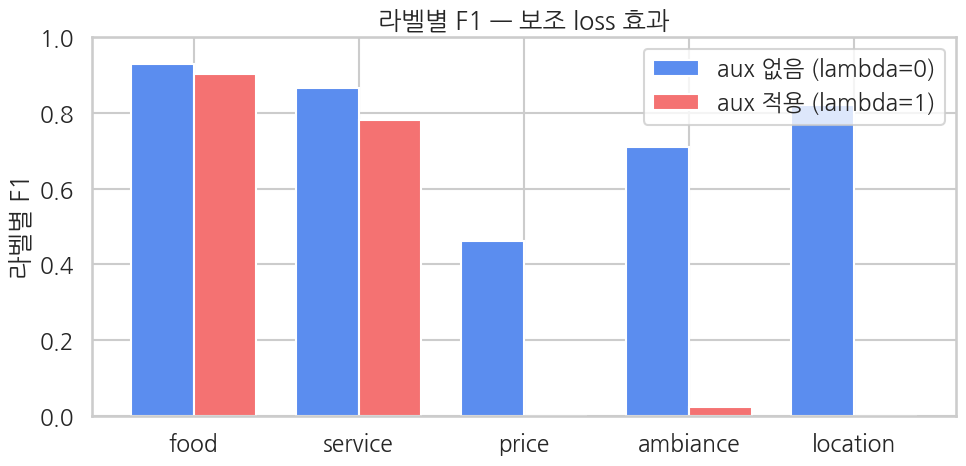
\includegraphics[width=0.88\linewidth]{assets/figures/ch14_aux_f1_compare.png}
\end{bookfigurelabel}



\textbf{해석}

\begin{itemize}
\tightlist
\item
  \textbf{별점과 상관이 강한 측면} (food, service): 보조 별점 회귀 학습이 \emph{긍정/부정 신호} 를 잘 잡으면 도움이 됩니다. 작은 양의 delta 기대.
\item
  \textbf{별점과 상관이 약한 측면} (location, price): 별점 신호가 \emph{직접적 도움} 이 안 됨. delta가 0 근처거나 약간 음수일 수 있음.
\item
  \textbf{분산이 큰 라벨} --- eval 표본이 적어 F1 자체가 노이즈가 큼. delta 도 의미 해석 조심.
\end{itemize}



\subsection{보조 태스크 평가}

별점 회귀가 잘 됐다는 건 BERT 본체가 \emph{별점 신호도 효율적으로 인코딩} 하고 있다는 뜻 --- 메인 task 표현에도 그 신호가 들어가 있을 가능성.



\Needspace{26\baselineskip}
\begin{lstlisting}
true_star = np.round(np.array(aux_true) * 4).astype(int) + 1
star_label = [f"{s}*" for s in true_star]
df_aux = pd.DataFrame({"True star": star_label, "Predicted (0-1 scale)": aux_preds_aux})
order = ["1*", "2*", "3*", "4*", "5*"]

fig, ax = plt.subplots(figsize=(8.5, 5.5))
sns.violinplot(
    data=df_aux, x="True star", y="Predicted (0-1 scale)",
    order=order, inner="quart", cut=0,
    color="#F47272", alpha=0.6, ax=ax,
)

for i, target in enumerate([0.0, 0.25, 0.5, 0.75, 1.0]):
    ax.hlines(
        target,
        i - 0.4,
        i + 0.4,
        color="black",
        lw=1.1,
        ls="--",
        alpha=0.7,
    )
ax.set_ylim(-0.2, 1.2)
ax.set_title(f"Aux task — predicted vs true star  (RMSE={rmse_aux:.3f}, r={pear_aux:.3f})")
plt.tight_layout()
plt.show()
\end{lstlisting}

\begin{bookfigurelabel}[htbp]{보조 별점 회귀 헤드의 예측 분포}{fig:ch14-aux-star-violin}
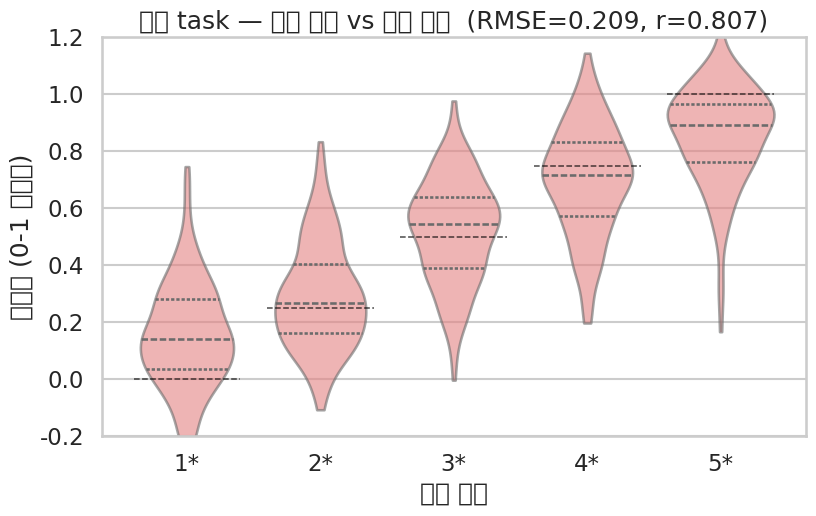
\includegraphics[width=0.82\linewidth]{assets/figures/ch14_aux_star_violin.png}
\end{bookfigurelabel}



\textbf{해석}

\begin{itemize}
\tightlist
\item
  각 violin이 \emph{해당 별점의 정답 위치} (점선 가이드: 1★=0.0, 2★=0.25, 3★=0.5, 4★=0.75, 5★=1.0) 에 \emph{중심} 하면 보조 head 가 별점 신호를 잘 학습한 것.
\item
  violin 의 \emph{너비} = 그 별점 내 예측 분산. 너비가 좁을수록 모델이 자신 있게 회귀 --- 모든 별점에서 좁으면 calibration 이 좋음.
\item
  가장 어려운 별점은 보통 \emph{3★} (중간값) --- 사람도 모호한 평가라 violin 이 길게 늘어지거나 인접 별점 위치까지 침범하면 자연스러움.
\item
  1★/5★ 양 끝 violin 이 정답 위치에서 \emph{체계적으로 안쪽} 으로 치우치면 \emph{극단값에 보수적} 인 회귀 --- MSE 가 양 끝에서 손실이 작아지는 특성과 결부된 일반적 경향.
\end{itemize}



\section{이 장에 등장한 라이브러리·함수}

\begin{booktable}{14장 새로 등장한 라이브러리}{tab:ch14-07}
\begin{adjustbox}{max width=\textwidth}
\begin{tabular}{@{}lll@{}}
\toprule
이름 & 한 줄 설명 & 다음 장에서 \\
\midrule

\inlinecode{Trainer.compute\_loss} 오버라이드 & 자동 매핑이 못 다루는 \emph{복합 loss} 직접 계산 & 18장 한국어 auxiliary 에서 다시 \\
\inlinecode{model.aux\_head\ =\ nn.Linear(...)} 한 줄 추가 & 표준 BERT 모델에 보조 헤드 동적 부착 & 18장 \\
\inlinecode{output\_hidden\_states=True} & 마지막 layer hidden 까지 받아 보조 헤드 입력으로 사용 & 보조 헤드 패턴마다 \\
\inlinecode{remove\_unused\_columns=False} & model.forward 시그니처에 없는 컬럼(aux\_labels)을 자동 제거 안 함 & custom collator 패턴마다 \\
커스텀 \inlinecode{DataCollator} & input\_ids 외 \emph{추가 라벨} 도 batch에 같이 담기 & 18장 \\
\inlinecode{r2\_score}, \inlinecode{np.corrcoef} & 회귀 task 보조 metric (R², Pearson r) & 회귀 결합 task 마다 \\
\bottomrule
\end{tabular}
\end{adjustbox}
\end{booktable}



\section{체크포인트 질문}

\begin{enumerate}
\def\labelenumi{\arabic{enumi}.}
\tightlist
\item
  λ를 0.1에서 10까지 grid search한다고 할 때 \emph{작은 λ} 와 \emph{큰 λ} 가 각각 어떤 학습 양상을 만드는지 한 줄로 설명하세요.
\item
  \inlinecode{remove\_unused\_columns=False} 를 빠뜨리면 어떤 에러가 나나요? \inlinecode{aux\_labels} 가 어디로 사라지는지 추적해 보세요.
\item
  보조 헤드의 파라미터가 \textasciitilde770개에 불과한데도 모델이 \emph{공유 본체} 학습에 영향을 주는 이유는?
\item
  메인 metric의 delta가 \emph{음수} 로 나왔다면 무엇을 의심해야 하고 어떻게 처치하나요?
\end{enumerate}



\section{FAQ}

\begin{faqBox}{Q1. (실무) λ는 어떻게 정하나요? 단순히 1.0으로 두면 되나요?}

1.0은 \emph{시작점} 일 뿐 거의 항상 grid search가 필요합니다.

\Needspace{12\baselineskip}
\begin{lstlisting}
for lam in [0.1, 0.3, 1.0, 3.0, 10.0]:
    trainer = AuxTrainer(..., lambda_aux=lam)
    trainer.train()
    metrics = trainer.evaluate()
    print(
        f"lambda={lam}: macro_f1="
        f"{metrics['eval_macro_f1']:.4f}"
    )
\end{lstlisting}

흔한 패턴:

\begin{itemize}
\tightlist
\item
  메인 task가 분류, 보조가 회귀 → λ=0.1-1.0 (회귀 MSE는 보통 분류 BCE 보다 작아 균형이 자연스러움)
\item
  메인이 복잡하고 보조가 \emph{미세} 보조 → λ=0.01-0.1
\item
  메인과 보조가 비슷한 중요도 → λ=1.0
\end{itemize}

또 다른 패턴: \textbf{uncertainty weighting} --- λ를 \emph{학습 가능한 파라미터} 로 두고 모델이 직접 결정하게 함 (Kendall et al. 2018).

\end{faqBox}

\begin{faqBox}{Q2. (이론) \inlinecode{outputs.loss} 는 BCE per-label 평균인데 왜 \emph{우리가 따로} 계산 안 하나요?}

\inlinecode{AutoModelForSequenceClassification} 의 forward 가 \inlinecode{problem\_type="multi\_label\_classification"} 와 \inlinecode{labels} 를 보고 \emph{자동으로} \inlinecode{BCEWithLogitsLoss(logits,\ labels)} 를 계산해 \inlinecode{outputs.loss} 에 담기 때문입니다.

\Needspace{24\baselineskip}
\begin{lstlisting}
class DistilBertForSequenceClassification:
    def forward(self, ..., labels=None):
        logits = self.classifier(self.pre_classifier(hidden))
        loss = None
        if labels is not None:
            if self.config.problem_type == "multi_label_classification":
                loss = F.binary_cross_entropy_with_logits(
                    logits,
                    labels.float(),
                )
            elif self.config.problem_type == "single_label_classification":
                loss = F.cross_entropy(logits, labels)
            elif self.config.problem_type == "regression":
                loss = F.mse_loss(
                    logits.squeeze(),
                    labels.float(),
                )
        return SequenceClassifierOutput(
            loss=loss,
            logits=logits,
            ...,
        )
\end{lstlisting}

우리는 \emph{메인 loss는 자동으로 받고, 보조 loss만 직접 계산해 더하면} 됩니다. 깔끔.

\end{faqBox}

\begin{faqBox}{Q3. (실무) 보조 헤드의 가중치는 사전학습이 안 되어 있는데 그래도 잘 학습되나요?}

네. 이유:

\begin{enumerate}
\def\labelenumi{\arabic{enumi}.}
\tightlist
\item
  \emph{작은 분류 헤드} 는 보통 사전학습 없이 random init 부터 시작해도 fine-tune 동안 충분히 빠르게 학습됩니다 (몇백 step 안에).
\item
  보조 헤드 위에 가중치가 \textasciitilde770개라 데이터에 \emph{과적합} 할 위험도 적습니다.
\item
  BERT 본체(67M)는 이미 표상이 풍부해 작은 head가 \emph{읽어내기만} 하면 됨.
\end{enumerate}

대조적으로 \emph{BERT 본체를 random init 부터} 학습하려면 수백 GB 데이터가 필요합니다. 사전학습 + 작은 head fine-tune 패턴이 강력한 이유.

\end{faqBox}

\begin{faqBox}{Q4. (이론) 보조 task가 메인과 \emph{반대 방향} 신호면 학습이 망가지나요?}

네, 정확히 그렇습니다. 예시:

\begin{itemize}
\tightlist
\item
  메인: 측면 분류 (긍정 측면 vs 부정 측면)
\item
  보조: \emph{반대로} 라벨링된 별점 (1★=좋음, 5★=나쁨 --- 라벨링 실수 시나리오)
\end{itemize}

이 경우 두 task의 gradient가 BERT 본체에서 \emph{반대 방향} 으로 끌어당겨 학습이 \emph{발산} 하거나 \emph{느려집니다}. 진단 신호:

\begin{itemize}
\tightlist
\item
  두 task의 train loss 가 \emph{둘 다 정체} (서로 상쇄)
\item
  λ 를 키울수록 메인 metric 이 \emph{떨어짐}
\end{itemize}

해결: 보조 task가 메인과 같은 방향 신호인지 \emph{간단한 sklearn baseline} 부터 확인. 별점이 측면 분류와 양의 상관이면 보조로 쓸 만함.

\end{faqBox}

\begin{faqBox}{Q5. (실무) 보조 task로 어떤 신호를 쓰는 게 좋나요?}

좋은 보조 task의 조건:

\begin{booktable}{14장 FAQ 표}{tab:ch14-08}
\begin{adjustbox}{max width=\textwidth}
\begin{tabular}{@{}ll@{}}
\toprule
좋은 조건 & 예시 \\
\midrule

\emph{메인과 양의 상관} & 측면 분류 ↔ 별점, 감성 분류 ↔ 이모지 사용 \\
\emph{학습 데이터가 \emph{공짜로} 있음} & 메타데이터(별점, 작성일, 길이) --- 라벨링 비용 0 \\
\emph{연속적이고 안정적인 신호} & float regression, 순서형 점수 \\
\emph{메인보다 \emph{덜 복잡} 한 task} & 회귀 \textless{} 분류, 단어 vs 문장 \\
\bottomrule
\end{tabular}
\end{adjustbox}
\end{booktable}

피해야 할 보조:

\begin{itemize}
\tightlist
\item
  메인보다 \emph{복잡한} task (예: 분류에 \emph{생성} 보조) --- 학습 비용 폭증
\item
  \emph{드물게 등장하는} 라벨 --- 학습 신호 부족
\item
  \emph{중복} 라벨 (메인과 거의 같은 정보) --- 추가 정보 없음
\end{itemize}

\end{faqBox}

\begin{faqBox}{Q6. (실무) 보조 task가 \emph{test 환경에서는 정답이 없는} 라벨이면 어떻게 활용하나요?}

학습 시에만 보조 라벨 사용, 추론 시에는 메인 head만 사용 --- \emph{학습 정규화} 용. 이게 auxiliary loss 의 \emph{정통 사용 패턴} 입니다.

\Needspace{9\baselineskip}
\begin{lstlisting}
trainer.train()

with torch.no_grad():
    out = model(input_ids=..., output_hidden_states=False)
    main_probs = torch.sigmoid(out.logits)
\end{lstlisting}

훈련 데이터에만 있는 \emph{부가 신호} (운영 시엔 사라지는 메타데이터)를 학습 시 활용하는 좋은 트릭.
\end{faqBox}



\section{오류 실험 (선택)}

다음 코드를 돌려보면 어떤 에러가 날까요?

\Needspace{10\baselineskip}
\begin{lstlisting}
training_args = TrainingArguments(
    ...,
    remove_unused_columns=True,
)
trainer = AuxTrainer(...)
trainer.train()
\end{lstlisting}

힌트: Trainer 가 \inlinecode{aux\_labels} 를 \emph{자동 제거} 한 뒤 우리 \inlinecode{compute\_loss} 안에서 \inlinecode{inputs.pop("aux\_labels")} 가 KeyError. \inlinecode{aux\_labels} 가 어디서 사라지는지 추적해 보면 학습 inputs 가 model.forward 시그니처와 맞춰지는 구조를 이해하게 됩니다.



\begin{previewBox}{미리보기: 다음 장}

\textbf{15장. BERT 한국어 Binary --- NSMC}

\begin{itemize}
\tightlist
\item
  Phase 1 영어(DistilBERT) → Phase 2 한국어(klue/bert-base) 전환
\item
  데이터: 네이버 영화 리뷰 (NSMC) 이진 분류 (긍정/부정)
\item
  셋업: \inlinecode{num\_labels=2} + \inlinecode{problem\_type="single\_label\_classification"} (\ref{ch:11}장과 같은 표준 binary 셋업)
\item
  변하는 축: \emph{언어 + 데이터 + 토크나이저} (영어 WordPiece → 한국어 WordPiece). 모델 크기는 비슷, 셋업도 같음.
\item
  회귀 장은 \emph{생략} (영어 \ref{ch:09}장 에서 다뤘으므로). Phase 2는 Binary 부터 시작.
\end{itemize}

\begin{quote}
\textbf{Phase 1 마무리} --- \ref{ch:07}--\ref{ch:14}장를 통해 BERT 분류·회귀·multi-label·auxiliary loss의 기본 5가지를 다 익혔습니다. Phase 2는 같은 패턴을 \emph{한국어 데이터} 위에서 압축적으로 재방문 --- 토크나이저가 어떻게 다른지, 한국어 특유의 학습 어려움이 무엇인지 확인.
\end{quote}
\end{previewBox}
